\documentclass[9pt,xcolor=pdftex,dvipsnames,table]{beamer} 
\setbeamercolor{bgcolor}{fg=white,bg=blue!100}
\mode<presentation>
{
  \usetheme{Darmstadt}
 \setbeamertemplate{navigation symbols}{}
  \setbeamercovered{transparent}
  \setbeamertemplate{footline}
{\rightline{\insertframenumber/\inserttotalframenumber}}
}

\def\newblock{}

\newenvironment{changemargin}[2]{% 
  \begin{list}{}{% 
    \setlength{\topsep}{0pt}% 
    \setlength{\leftmargin}{#1}% 
    \setlength{\rightmargin}{#2}% 
    \setlength{\listparindent}{\parindent}% 
    \setlength{\itemindent}{\parindent}% 
    \setlength{\parsep}{\parskip}% 
  }% 
  \item[]}{\end{list}} 
  
\usepackage[english]{babel}
\usepackage{amsmath}
\usepackage{lipsum}
\usepackage[latin1]{inputenc}
\usepackage{times}
\usepackage[latin1]{inputenc}
\usepackage{tipa}
\usepackage{color}
\usepackage{ulem}
\usepackage{booktabs}
\usepackage{colortbl}
\usepackage{listings}
\usepackage{gb4e}
\usepackage{longtable}
\usepackage{pgf,pgfarrows,pgfnodes}
\usepackage{tikz} 
\usepackage{textpos}            % free image positioning 
\setlength{\TPVertModule}{1cm}  % unit for vertical positioning 
\setlength{\TPHorizModule}{1cm} % unit for horizontal positioning 

\definecolor{lightorange}{rgb}{1,0.75,.25}
\definecolor{lightred}{rgb}{1,0.25,.25}
\definecolor{lightblue}{rgb}{.25,.25,1.0}
\definecolor{lightgray}{rgb}{.75,.75,.75}

\usepackage[T1]{fontenc}

\title{N-Grams Episode I: Counting}
\author{Linguistics 409 $\cdot$ Computational Linguistics}
\date[]{}
\usepackage{gb4e}

\usepackage{natbib}
\bibliographystyle{apalike}

\makeatletter
\newcommand\textsubscript[1]{\@textsubscript{\selectfont#1}}
\def\@textsubscript#1{{\m@th\ensuremath{_{\mbox{\fontsize\sf@size\z@#1}}}}}
\newcommand\textbothscript[2]{%
  \@textbothscript{\selectfont#1}{\selectfont#2}}
\def\@textbothscript#1#2{%
  {\m@th\ensuremath{%
    ^{\mbox{\fontsize\sf@size\z@#1}}%
    _{\mbox{\fontsize\sf@size\z@#2}}}}}
\def\@super{^}\def\@sub{_}
\makeatother

\begin{document}
\definecolor{grey}{rgb}{1,0.6,.7}

\section{Introduction to N-grams}

\begin{frame}

	\titlepage
	\begin{center}
		\vspace{-1.5cm}
		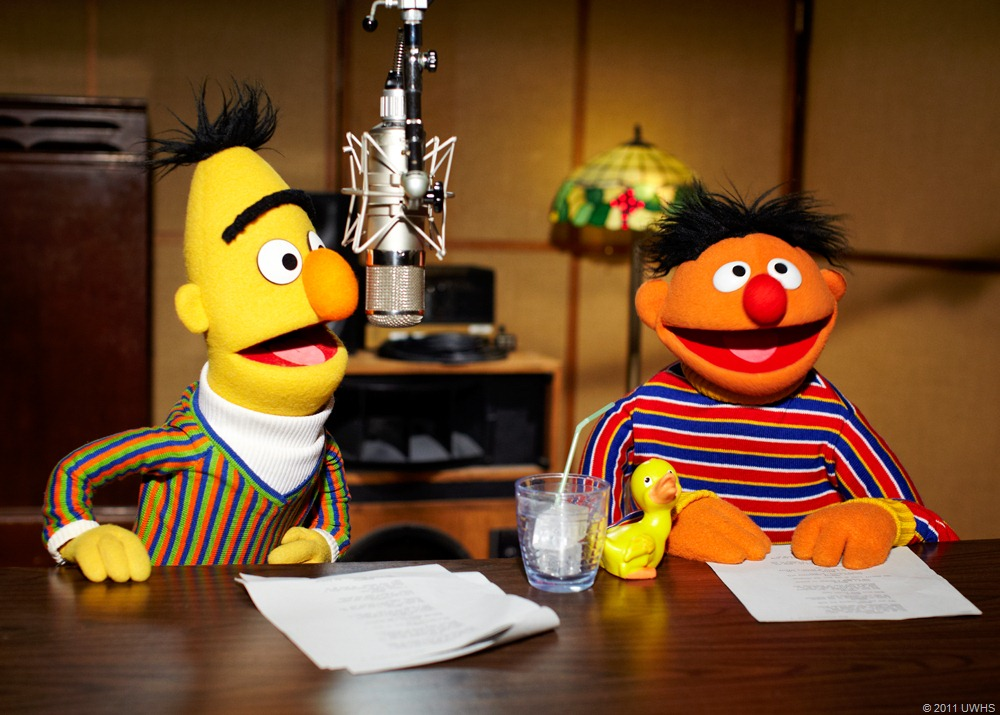
\includegraphics[width=.5\paperwidth]{Bert-Ernie}	
	\end{center}
\end{frame}

\subsection{}
\begin{frame}{Word Prediction}

	\begin{itemize}
		\item Guess the next word...
		\item ``I notice three guys standing on the ???''
		\item Many sources of knowledge can be used to inform this task, including world knowledge.
		\item Prediction can be quite good simply by looking at the
preceding words and keeping track of some fairly simple counts.
	\end{itemize}
\end{frame}

\subsection{}
\begin{frame}{Word Prediction}

	\begin{itemize}
		\item We can formalize this task using what are called \textbf{N-gram} models.
		\item N-grams are sequences of tokens.  The N indicates the length of the sequence.
		\item The previous example contains the following 2-grams (bigrams)
		\item (I notice), (notice three), (three guys), (guys standing),
(standing on), (on the)
		\item Given knowledge of counts of N-grams such as these, we can
guess likely next words in a sequence.
	\end{itemize}
\end{frame}

\subsection{}
\begin{frame}{N-Gram Models}

	\begin{itemize}
		\item Somewhat more formally:
		\item We can use knowledge of the counts of N-grams to assess the conditional probability of candidate words as the next word in a sequence.
		\item Or, we can use them to assess the probability of an entire sequence of words.
		\item These are pretty much the same task as we'll see...
	\end{itemize}
\end{frame}

\subsection{}
\begin{frame}{Applications}

{\large It turns out that being able to predict the next word (or morpheme, or phoneme, or diphone, etc.) in a sequence is an extremely useful thing to
be able to do.  It's central to:}

	\begin{itemize}
		\item Automatic speech recognition
		\item Handwriting and character recognition
		\item Spelling correction
		\item Machine translation
		\item NLP: POS Tagging, NL generation, Authorship, Sentiment analysis,
predictive text
	\end{itemize}
\end{frame}

\subsection{}
\begin{frame}{Relevant XKCD}
	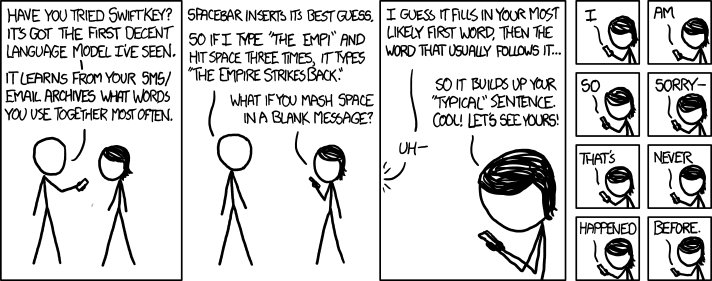
\includegraphics[width=.85\paperwidth]{swiftkey}	
\end{frame}

\section{Counting}

\subsection{}
\begin{frame}{Remember our working definition...}

\vspace{.5cm}
     \begin{itemize}
          \item Recall that the probability of an event e is computed as the relative frequency with which $e$ occurs in a sequence of $n$ identical experiments:
          \item The probability $P$ of an event $e$ is computed as:
          
          	\begin{equation*}{P(e) = \frac{n_e}{n}}\end{equation*}
          
          \item $n_e$ is the number of occurrences of the event $e$ in $n$ identical experiments.
     \end{itemize}\pause
     
	\vspace{.25cm}
	
	{\large If the event $e$ is a single word in a corpus then $P(e) = \frac{n_e}{n}$ is a 1-gram or \textbf{unigram} probability.}\pause

	\vspace{.25cm}
	
	{\large If the event $e$ is a pair of words in a corpus then $P(e) = \frac{n_e}{n}$ is a 2-gram or \textbf{bigram} probability.}
\end{frame}

\subsection{}
\begin{frame}{Counting Bigrams}

{\large As you'll recall, simple counting lies at the core of any probabilistic approach. So let's take a look at what we're counting.}

\vspace{.25cm}

{\huge \textbf{He put the ring in his pocket almost without thinking: certainly it did not seem of any particular use at the moment.}}

\vspace{.25cm}

	\begin{itemize}
		\item 22 tokens or 24 if we include ``:'' and ``,'' as separate tokens.\pause
		\item Assuming we include the punctuation, how many bigrams are there?
	\end{itemize}
\end{frame}

\subsection{}
\begin{frame}{It's not always that simple...}

{\large ``the uh um uh uh oh what's it called the uh uh the post... the posterior probability!''}

\vspace{.25cm}

	\begin{itemize}
		\item Should we count \emph{uh} and other disfluencies as tokens?
		\item The answers depend on the application!
		\item What about the fragment as in `posterior'? Should such do-overs count twice or just once?
		\item If we're focusing on something like ASR to support indexing for search, then \emph{uh} probably isn't helpful (it's unlikely to occur as a query).
		\item But filled pauses are very useful in dialog management, so we might need them.
	\end{itemize}
\end{frame}

\subsection{}
\begin{frame}{For next time:}

     \begin{block}{For next time:}
          \begin{enumerate}
               \item Monday: \textbf{More N-Grams!}
               \item Start HW2!
               \item Read Chapter 4 pp 97 - 109 
          \end{enumerate}
     \end{block}
\end{frame}

\subsection{}
\begin{frame}{Types and tokens}

{\large ``There is nothing like looking, if you want to find something. You certainly usually find something, if you look, but it is not always quite the something you were after.''}

\vspace{.25cm}

	\begin{itemize}
		\item 30 tokens.\pause
		\item But notice that \emph{you} is repeated 4 times, \emph{something} is repeated 3 times, \emph{is}, \emph{if}, and \emph{find} are repeated twice each, and 17 other words are repeated once each. \pause
		\item This means there are 30 tokens but 22 \textbf{types}. \pause
		\item What is the unigram probability of the type \emph{you} in this text ($P(you)$)?  What is $P(always)$?
	\end{itemize}
\end{frame}

\subsection{}
\begin{frame}{Types and tokens}

{\large ``There is nothing like looking, if you want to find something. You certainly usually find something, if you look, but it is not always quite the something you were after.''}

\vspace{.25cm}

	\begin{itemize}
		\item How would you get these type \& token counts for an arbitrarily large corpus using UNIX commands?\pause
		\item Note how important tokenization becomes.  Does punctuation figure into our bigram probabilities? \pause
		\item Incidentally, what is the 10th bigram in this text?
	\end{itemize}
\end{frame}

\subsection{}
\begin{frame}{Lemmas \& Wordforms}

{\large ``There is nothing like looking, if you want to find something. You certainly usually find something, if you look, but it is not always quite the something you were after.''}

\vspace{.125cm}

	\begin{itemize}
		\item Should \emph{looking} and \emph{look} count as the same when we are counting?
		\item How about \emph{is} and \emph{were}?
		\item Or, in another text, \emph{goose} and \emph{geese}?
\end{itemize}\pause

\vspace{.125cm}

	\begin{description}
		\item[\textbf{Lemma}] a set of lexical forms having the same stem, major part of speech, and word sense
		\item[\textbf{Wordform}] a fully inflected surface form
	\end{description}

\vspace{.125cm}

	\begin{itemize}
		\item Again, we'll have occasion to count both lemmas and wordforms in compling.
	\end{itemize}
\end{frame}

\subsection{}
\begin{frame}{Let's try it...}

{\large Buffalo buffalo buffalo Buffalo buffalo.}

\vspace{.25cm}

	\begin{itemize}
		\item How many tokens?
		\item How many types?
		\item What kind of linguistic knowledge would a parser need to generate these counts accurately?  What other kinds of knowledge?
	\end{itemize}
\end{frame}


\subsection{}
\begin{frame}{Corpora}

{\large Brown Corpus (Kucera \& Francis 1967) }\\
\url{http://archive.org/details/BrownCorpus}

\vspace{.25cm}

\begin{columns}
    \begin{column}[t]{0.4\textwidth}
	\begin{itemize}
		\item 1,014,312 tokens
		\item 55,106 types
	\end{itemize}
	\end{column}
	
	\begin{column}[t]{0.6\textwidth}
	
	\begin{exampleblock}{Top 10 types in Brown Corpus}
	
		\begin{itemize}
			\item[] 62,713 the
			\item[] 36,080 of
			\item[] 27,932 and
			\item[] 25,732 to
			\item[] 21,881 a
			\item[] 19,536 in
			\item[] 10,237 that
			\item[] 10,011 is
			\item[] 9,777 was
			\item[] 8,841 for
		\end{itemize}
	\end{exampleblock}
	
	\end{column}
\end{columns}
\end{frame}

\begin{frame}{Corpora}

{\large Google 5-Grams Corpus }\\
\url{http://googleresearch.blogspot.com/2006/08/all-our-n-gram-are-belong-to-you.html}

\vspace{.25cm}

\begin{columns}
    \begin{column}[t]{0.4\textwidth}
	\begin{itemize}
		\item 1,024,908,267,229 tokens*
		\item 13,588,391 types*
	\end{itemize}
	\vspace{1cm}
	* counts are for published 2006 LDC corpus.
	\end{column}
	
	\begin{column}[t]{0.6\textwidth}
	
	\begin{exampleblock}{Interactive N-Gram Viewer}
	
		As part of their Google Books product, Google makes available the interactive (and addictive) N-Grams viewer:
		
		\url{http://books.google.com/ngrams}
	\end{exampleblock}
	
	\end{column}
\end{columns}
\end{frame}

\section{Language Modelling}

\subsection{}
\begin{frame}{Language Modelling}

	\begin{itemize}
		\item Let's get back to word prediction!
		\item We can model the word prediction task as the ability to assess the conditional probability of a word given the previous words in the sequence.
		
			\vspace{.3cm}
			\begin{equation*}P( wn | w1,w2...w^{n-1} )\end{equation*}
			\vspace{.2cm}
						
		\item We'll call a statistical model that can assess this conditional probability a \textbf{Language Model}.
	\end{itemize}
\end{frame}

\subsection{}
\begin{frame}{Language Modelling}

	\begin{itemize}
		\item How might we go about calculating such a conditional
probability?
		\item One way is to use the definition of conditional probabilities and look for counts. So to get:
		
		\begin{equation*}P(the | its\,water\,is\,so\,transparent\,that)\end{equation*}
		
		\item By definition that's:

		\begin{equation*}\frac{P(its\,water\,is\,so\,transparent\,that\,the)}{P(its\,water\,is\,so\,transparent\,that)}
		\end{equation*}

		\item In theory we can get each of those from counts from a sufficiently large corpus.

	\end{itemize}
\end{frame}

\subsection{}
\begin{frame}{Easily estimated...}

	\begin{itemize}
		\item  The \textbf{maximum likeliehood estimation} (MLE) for the probability of a particular string in a corpus is simply the number of times that string occurs divided by the number of opportunities it \emph{had} to occur. 
	\end{itemize}
			
		\begin{equation*}P(the | its\,water\,is\,so\,transparent\,that) = \frac{Count(its\,water\,is\,so\,transparent\,that\,the)}{Count(its\,water\,is\,so\,transparent\,that)}
		\end{equation*}
\end{frame}

\subsection{}
\begin{frame}{Language Modelling}

	\begin{itemize}
		\item  Alas, in practice we are unlikely to get good estimates from this method.
		\item What we're likely to get is 0. Or worse 0/0!
		\item Clearly, we'll have to be cleverer.
		\item Let's use the chain rule of probability and a particularly useful\footnote{though, strictly speaking, wrong.} independence assumption.
	\end{itemize}
\end{frame}

\subsection{}
\begin{frame}{Recall: the Chain Rule}

Earlier, we introduced the \textbf{chain rule}:

\begin{equation*}
	P(w_1,w_2,w_3,w_4,w_n) = P(w_1) x P(w_2|w_1) x P(w_3|w_2,w_1) x ... x P( w_n | w_{n-1}, w_{n-2},...,w_1)
\end{equation*}

This long product is usually expressed:

\begin{equation*}
	P(w_1,w_2,...,w_n) = \prod_{i=1}^{n} P( w_i | w_{i-1}, w_{i-2},...,w_1)
\end{equation*}

Jurafsky and Martin represent this: 

\begin{equation*}
	P(w_1,w_2,...,w_n) = \prod_{k=1}^{n} P( w_k | w^{k-1}_1)
\end{equation*}

\end{frame}


\subsection{}
\begin{frame}{Language Modelling}

\begin{equation*}
	P(w_1,w_2,...,w_n) = \prod_{k=1}^{n} P( w_k | w^{k-1}_1)
\end{equation*}
\vspace{.3cm}

	\begin{itemize}
		\item Estimate the joint probability of a sequence of words by multiplying together a number of conditional probabilities?
	\end{itemize}
	
\begin{equation*}
\begin{aligned}
P(its\,water\,was\,so\,transparent) &= \\
	&P(its) x P(water|its)\\
	&x\,P(was|its\,water) \\
	&x\,P(so|its\,water\,was) \\
	&x\,P(transparent|its\,water\,was\,so)
\end{aligned}
\end{equation*}
\end{frame}

\subsection{}
\begin{frame}{Independence Assumption}

{\large Instead of this:}

\begin{equation*}
	P(w_1,w_2,...,w_n) = \prod_{k=1}^{n} P( w_k | w^{k-1}_1)
\end{equation*}
\vspace{.3cm}

	\begin{itemize}
		\item let's assume that the probability of a word isn't dependent on \emph{every} preceding word in the phrase, sentence, document, or corpus...\pause
		\item let's try:
		
		\begin{equation*}P(the | its\,water\,is\,so\,transparent\,that) = \frac{Count(its)}{Count(its\,water)}
		\end{equation*}
		
		\item or:
		
		\begin{equation*}P(the | its\,water\,is\,so\,transparent\,that) = \frac{Count(its)}{Count(its\,water\,is)}
		\end{equation*}
	\end{itemize}
\end{frame}

\subsection{}
\begin{frame}{Independence Assumption}

\begin{columns}
	\begin{column}[T]{3cm}
	
	{\large This particular kind of independence assumption is called a \textbf{Markov} assumption after the famous Russian defenseman Andrei Markov. }
	\end{column}
	
	\begin{column}[T]{5.5cm}
		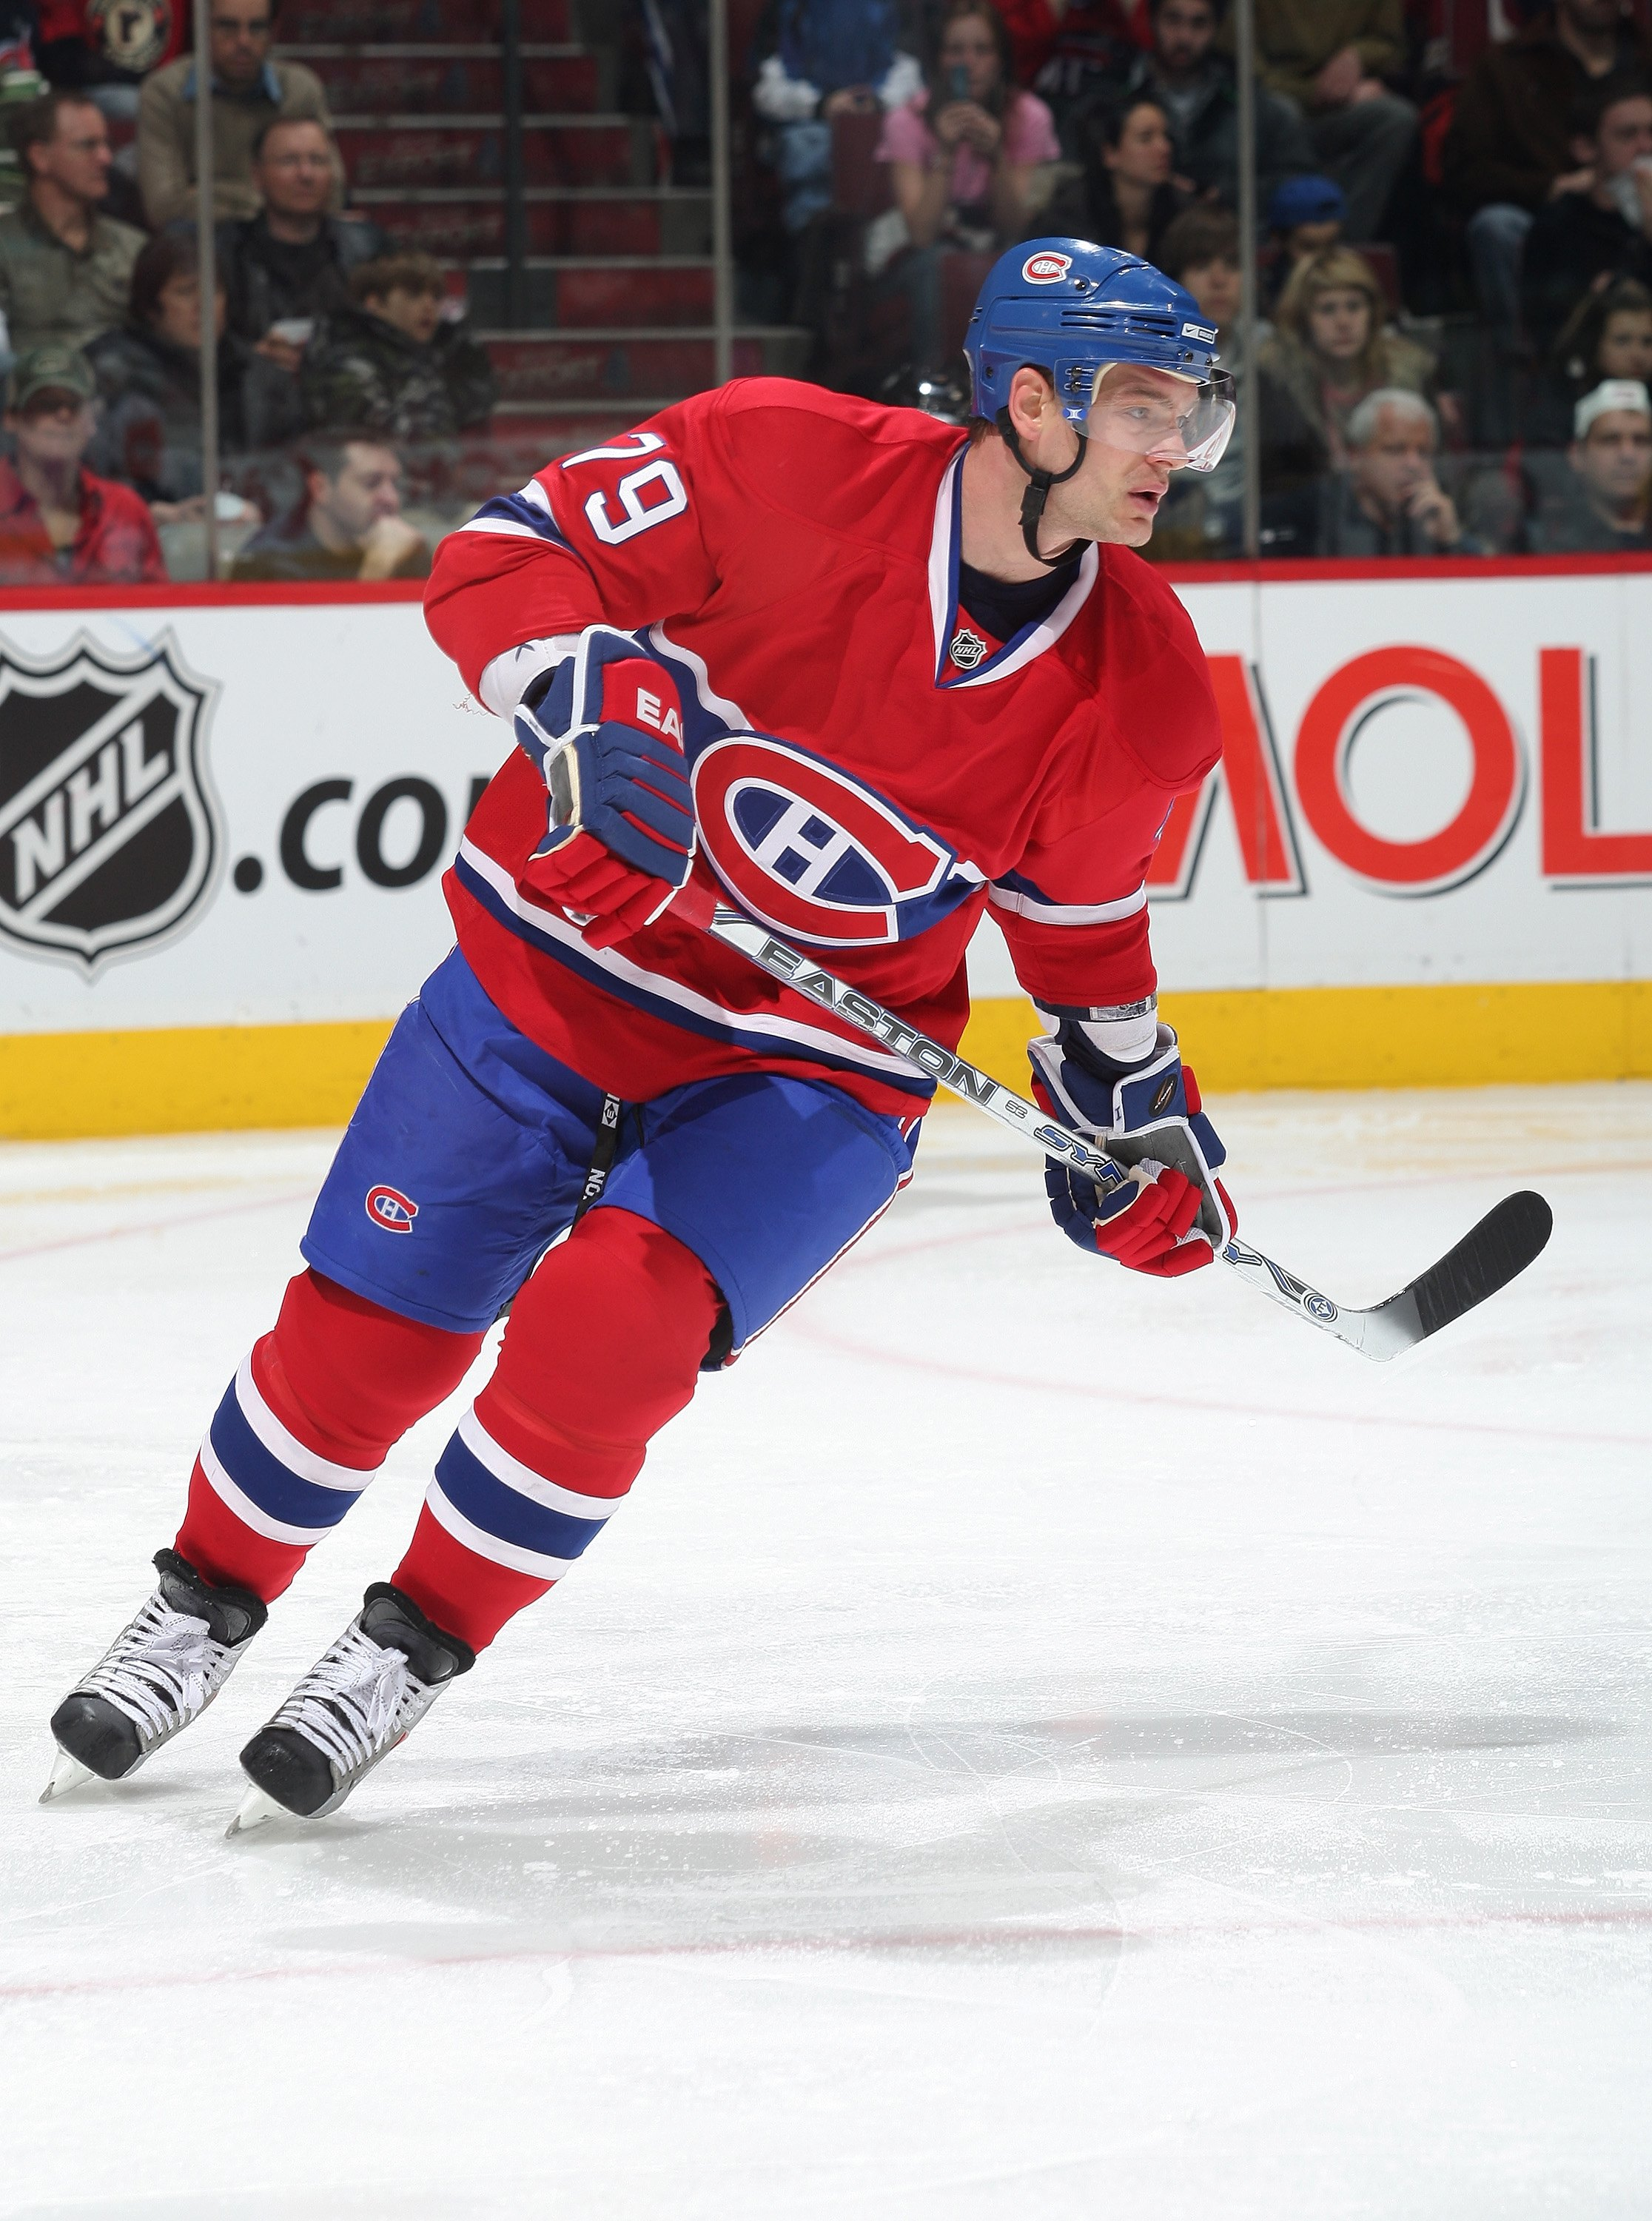
\includegraphics[width=5.5cm]{markov1}	
	\end{column}
\end{columns}
\end{frame}

\subsection{}
\begin{frame}{Independence Assumption}

\begin{columns}
	\begin{column}[T]{3cm}
	
	{\large This particular kind of independence assumption is called a \textbf{Markov} assumption after the famous Russian \sout{defenseman} mathematician Andrei Markov. }
	\end{column}
	
	\begin{column}[T]{5.5cm}
		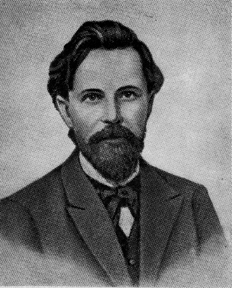
\includegraphics[width=5.5cm]{markov2}	
	\end{column}
\end{columns}
\end{frame}

\subsection{}
\begin{frame}{Markov Assumption}

{\large General idea: limit history to fixed number of words $N$}

\begin{equation*}
	P(w_n|w^{n-1}_1) \approx P(w_n|w^{n - 1}_{n - N + 1})
\end{equation*}
\vspace{.3cm}

{\large Bigram version}

\begin{equation*}
	P(w_n|w^{n-1}_1) \approx P(w_n|w_{n - 1})
\end{equation*}
\vspace{.3cm}

\end{frame}

\subsection{}
\begin{frame}{Estimating bigram probabilities}

{\large The bigram MLE is:}

\begin{equation*}
	P(w_n|w^{n-1}_1) = \frac{ Count(w_{n-1},w_n) }{ Count(w_{n-1}) }
\end{equation*}
\vspace{.3cm}
\end{frame}

\subsection{}
\begin{frame}[fragile]{Example: P(Seuss|Dr.)}

\begin{equation*}
	P(w_n|w^{n-1}_1) = \frac{ Count(w_{n-1},w_n) }{ Count(w_{n-1}) }
\end{equation*}
\vspace{.3cm}

\begin{lstlisting}[language=html]
	<s> I am Sam </s>
	<s> Sam I am </s>
	<s> I do not like green eggs and ham </s>
\end{lstlisting}

\begin{itemize}
	\item What are the bigrams?
	\item What are the line markers for?
	\item What is P(eggs|green)?
	\item What is P(Sam|<s>)?
	\item What is P(Sam|am)?
\end{itemize}
\end{frame}

\subsection{}
\begin{frame}{For next time:}

     \begin{block}{For next time:}
          \begin{enumerate}
               \item Wednesday: \textbf{Still More N-Grams!}
               \item Read Chapter 4 pp 97 - 109 
          \end{enumerate}
     \end{block}
\end{frame}

\begin{frame}{}
\begin{columns}
	\begin{column}[T]{3cm}
	
	{\huge Improbable Lobsters}
	\end{column}
	
	\begin{column}[T]{7cm}
		
\includegraphics[width=7cm]{lobster-cartoon}	
	\end{column}
\end{columns}
\end{frame}

\subsection{}
\begin{frame}[fragile]{Example: P(Seuss|Dr.)}

\begin{equation*}
	P(w_n|w^{n-1}_1) = \frac{ Count(w_{n-1},w_n) }{ Count(w_{n-1}) }
\end{equation*}
\vspace{.3cm}

\begin{lstlisting}[language=html]
	<s> I am Sam </s>
	<s> Sam I am </s>
	<s> I do not like green eggs and ham </s>
\end{lstlisting}

\begin{itemize}
	\item What are the bigrams?
	\item What are the line markers for?
	\item What is P(eggs|green)?
	\item What is P(Sam|<s>)?
	\item What is P(Sam|am)?
\end{itemize}
\end{frame}
\begin{frame}{Estimating bigram probabilities}

{\large The bigram MLE is:}

\begin{equation*}
	P(w_n|w^{n-1}_1) = \frac{ Count(w_{n-1},w_n) }{ Count(w_{n-1}) }
\end{equation*}

\vspace{1cm}

{\large This is the Maximum Likelihood Estimate, because it is the one
which maximizes $P(Training\,set|Model)$}

\end{frame}

\subsection{}
\begin{frame}{Maximum Likeliehood Estimates}

{\large The maximum likelihood estimate of some parameter of a
model $M$ from a training set $T$ is the estimate that maximizes the likelihood of the training set $T$ given the model $M$.}

\begin{itemize}
	\item Suppose the word \emph{lobster} occurs 42 times in a corpus of a million words (e.g. the Brown corpus)
	\item What is the probability that a random word from some other text from the same distribution will be \emph{lobster}?
	\item MLE estimate is 42/1,000,000 = 0.000042
	\item This is likely to be a terrible estimate for a travel book about Maine or a guide to seafood restaurants in Newfoundland, but it is the estimate that makes it most likely that \emph{lobster} will occur 42 times in a 1,000,000 word corpus.
	\item In other words, we're using the structure, genre, register, and content of a training corpus to make estimates about a test corpus.
\end{itemize}
\end{frame}

\subsection{}
\begin{frame}{More examples: Berkeley Restaurant Project sentences}

\begin{itemize}
	\item can you tell me about any good cantonese restaurants close by
	\item mid priced thai food is what i'm looking for
	\item tell me about chez panisse
	\item can you give me a listing of the kinds of food that are available
	\item i'm looking for a good place to eat breakfast
	\item when is caffe venezia open during the day
	\end{itemize}
\end{frame}

\subsection{}
\begin{frame}{Berkeley: Raw bigram counts ($Count(w_{n-1},w_n)$)}

	\begin{itemize}
		\item Out of 9,222 sentences
		\item e.g. ``I want'' occurred 827 times
	\end{itemize}
	
	\vspace{.5cm}
		
	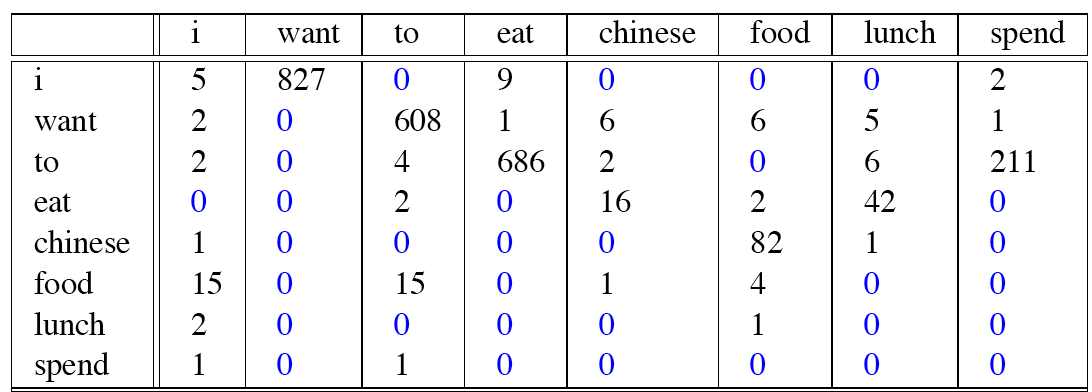
\includegraphics[width=.9\paperwidth]{berkeleyCounts}	
\end{frame}

\subsection{}
\begin{frame}{Berkeley: Normalize by unigrams ($Count(w_{n-1})$)}

	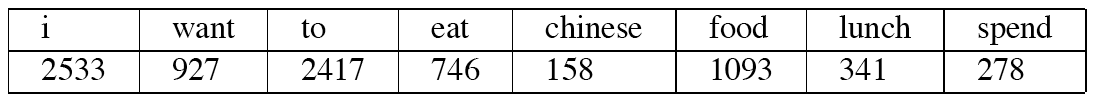
\includegraphics[width=.9\paperwidth]{berkeleyUnigrams}
	
	\vspace{.25cm}
		
	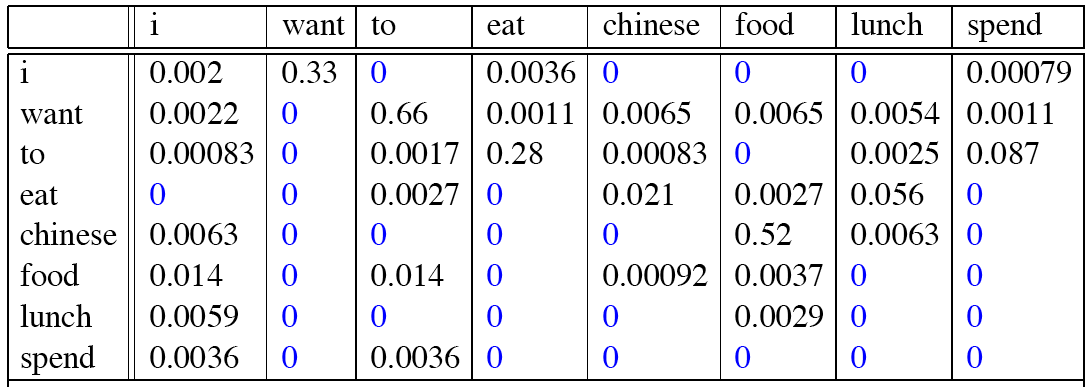
\includegraphics[width=.9\paperwidth]{berkeleyNormalized}
\end{frame}

\subsection{}
\begin{frame}{Berkeley: Bigram estimates of sentence probability}

{\large P(<s> I want english food </s>) = }
\begin{equation*}
\begin{aligned}
	& P( I | <s> )		\\
 	& x\,  P(want |I)  \\
	& x\,  P(english|want)	\\   
	& x\,  P(food|english)   	\\
	& x\,  P(</s>|food)		\\
    & =  .000031
\end{aligned}
\end{equation*}

{\large P(<s> I want chinese food </s>) =\\.25 x .33 x .0065 x .5 x .68 = 0.00018 }
\end{frame}

\subsection{}
\begin{frame}{What kinds of knowledge are we modelling?}

\begin{itemize}
	\item P(english|want) = .0011
	\item P(chinese|want) = .0065
	\item P(to|want) = .66
	\item P(eat | to) = .28
	\item P(food | to) = 0
	\item P(want | spend) = 0
	\item P (i | <s>) = .25
\end{itemize}
\end{frame}

\subsection{}
\begin{frame}{What kinds of knowledge are we modelling?}

\begin{itemize}
	\item P(english|want) = .0011
	\item P(chinese|want) = .0065
	\item P(to|want) = .66
	\item P(eat | to) = .28
	\item P(food | to) = 0
	\item P(want | spend) = 0
	\item P (i | <s>) = .25
\end{itemize}
\end{frame}

\section{Smoothing}

\subsection{}
\begin{frame}{Shannon's Visualization Method: N-Gram Generation}

\begin{columns}
	\begin{column}[T]{5.5cm}
		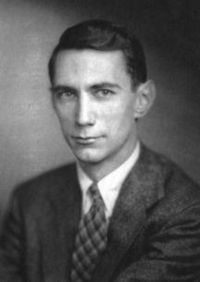
\includegraphics[width=5cm]{shannon}	
	\end{column}
	
	\begin{column}[T]{3cm}
	{\large Perhaps more interesting than assigning probabilities to sentences is turning the model around and using it to \textbf{generate random sentences} that are like the model sentences. This is typically attributed to Claude Shannon.}
	\end{column}
\end{columns}

\end{frame}

\subsection{}
\begin{frame}{Shannon's Visualization Method: N-Gram Generation}

\begin{enumerate}
	\item Sample a random bigram (<s>, w) according to its probability
	\item Sample a random bigram (w, x) according to its probability
	\item Repeat until we randomly choose a (z, </s>)
	\item String the words together:
\end{enumerate}

\begin{center}
\begin{tabular}{l l l l l l l l}
\textcolor{blue}{<s>} & \textcolor{blue}{I} &      &    &     &         &      &      \\
    & \textcolor{blue}{I} & want &    &     &         &      &      \\
    &   & \textcolor{blue}{want} & to &     &         &      &      \\
    &   &      & \textcolor{blue}{to} & eat &         &      &      \\
    &   &      &    & \textcolor{blue}{eat} & Chinese &      &      \\
    &   &      &    &     & \textcolor{blue}{Chinese} & food &      \\
    &   &      &    &     &         & \textcolor{blue}{food} & </s> \\
\end{tabular}
\end{center}
\end{frame}

\subsection{}
\begin{frame}{Generating Random Shakespeare}
\begin{center}
	\makebox[\linewidth]{\parbox{12.5cm}{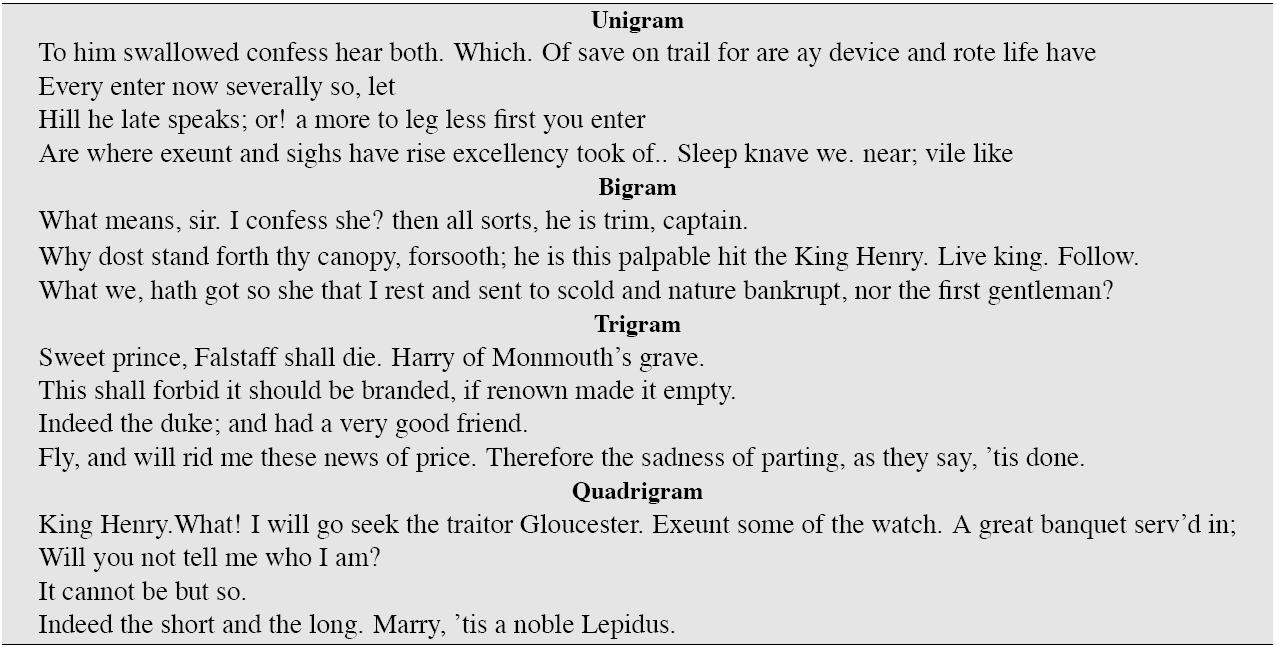
\includegraphics[width=12.5cm]{ngrams4-3}}}\\
	{\large J\&M Figure 4.3}\\
\end{center}
\end{frame}

\subsection{}
\begin{frame}{Shakespeare as Corpus}

\begin{itemize}
	\item 884,647 tokens but only 29,066 wordforms
	\item Shakespeare produced a mere 300,000 bigram types out of 844 million possible bigrams.
	\item So, 99.96\% of the possible bigrams are never seen (have zero entries in the table)
	\item This is the single biggest problem in language modelling.
	\item 4-grams are worse: what's coming out looks like Shakespeare because it is Shakespeare
	\item This is an expected property of Shannon visualization.
\end{itemize}
\end{frame}

\subsection{}
\begin{frame}{Generating Random Wall Street Journal}
\begin{center}
	\makebox[\linewidth]{\parbox{12.5cm}{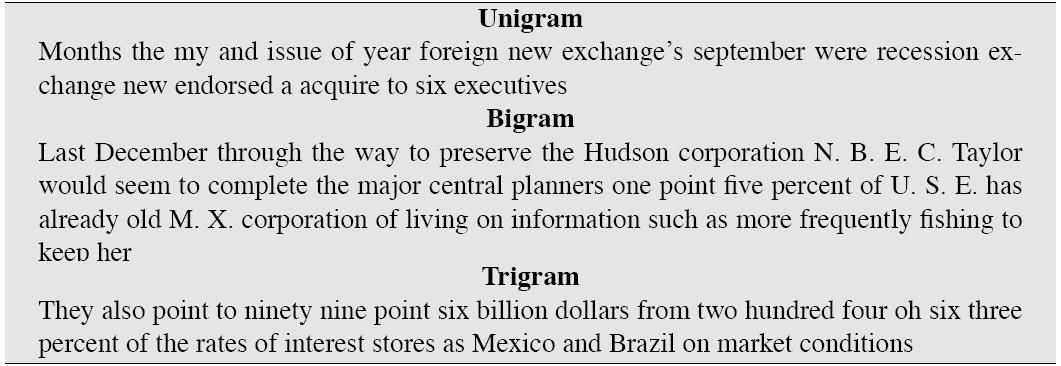
\includegraphics[width=12.5cm]{ngrams4-4}}}\\
	{\large J\&M Figure 4.4}\\
\end{center}
\end{frame}

\subsection{}
\begin{frame}{Lesson 1: The perils of overfitting}

\begin{itemize}
	\item N-grams only work well for word prediction if the test corpus looks like the training corpus
	\item If you train only on Dr. Seuss, your language model is useless for OCR (unless you're scanning Dr. Seuss!).
	\item We need to train robust models, adapt to test sets, etc.
	\item What does this mean for Google N-Grams?
\end{itemize}
\end{frame}

\subsection{}
\begin{frame}{Lesson 2: Real zeroes or not?}

{\large Some of those zeros are really zeros...}

\begin{itemize}
	\item Some things really don't happen (e.g. *Dog the bit fish my.)!
	\item On the other hand, some zeroes are just rare events.
	\item If the training corpus had been a little bigger they may have had a count
\end{itemize}
\end{frame}

\subsection{}
\begin{frame}{Lesson 2: zeroes or not?}

{\large Some of those zeros are really zeros...}

\begin{itemize}
	\item What would that count be in all likelihood?
	\item Zipf's Law (long tail phenomenon):
	\begin{itemize}
		\item A small number of events occur with high frequency
		\item A large number of events occur with low frequency
	\end{itemize}
	\item You can quickly collect statistics on the high frequency events
	\item You might have to wait an arbitrarily long time to get valid statistics on low frequency events
\end{itemize}
\end{frame}

\subsection{}
\begin{frame}{Lesson 2: zeroes or not?}

{\large Some of those zeros are really zeros...}

\begin{description}
	\item[Result] Our estimates are sparse! We have no counts at all for the vast bulk of things we want to estimate!
	\item[Answer] Estimate the likelihood of unseen (zero count) N-grams!
\end{description}
\end{frame}

\subsection{}
\begin{frame}{Smoothing away those zeroes}

	{\large We can fill in those zeroes by stealing probability mass from the rich and giving it to the poor.}
	\vspace{.5cm}
	
	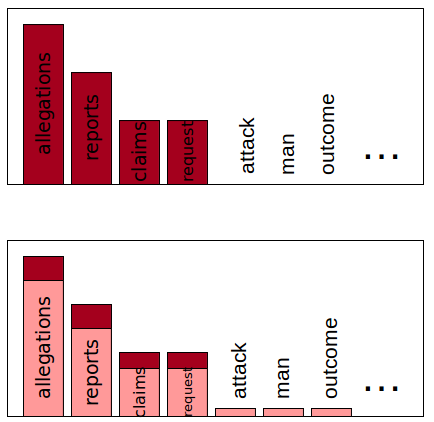
\includegraphics[width=6cm]{smoothing}	
\end{frame}

\subsection{}
\begin{frame}{Add-one smoothing}

	\begin{itemize}
		\item Also called Laplace Smoothing
		\item Pretend we saw each word one more time than we did
		\item Just add one to all the counts!
	\end{itemize}
	
	\vspace{.5cm}
		
	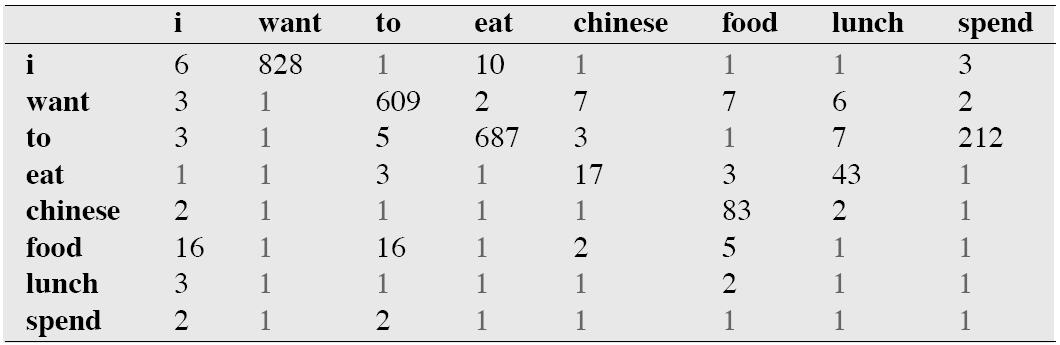
\includegraphics[width=.9\paperwidth]{ngrams4-5}	
\end{frame}

\subsection{}
\begin{frame}{Laplace-smoothed bigrams}

\begin{equation*}
	P^*(w_n|w^{n-1}_1) = \frac{ Count(w_{n-1},w_n) + 1 }{ Count(w_{n-1}) + V }
\end{equation*}

	\vspace{.5cm}
		
	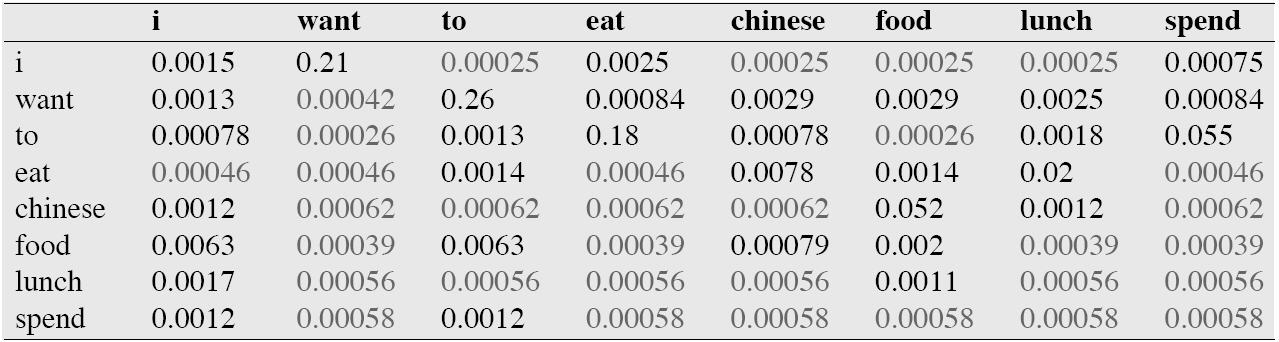
\includegraphics[width=.9\paperwidth]{ngrams4-6}	
\end{frame}

\subsection{}
\begin{frame}{Reconstituted counts}

\begin{equation*}
	Count^*(w_n|w^{n-1}_1) = \frac{ [Count(w_{n-1},w_n) + 1] Count(w_{n-1}) }{ Count(w_{n-1}) + V }
\end{equation*}

	\vspace{.5cm}
		
	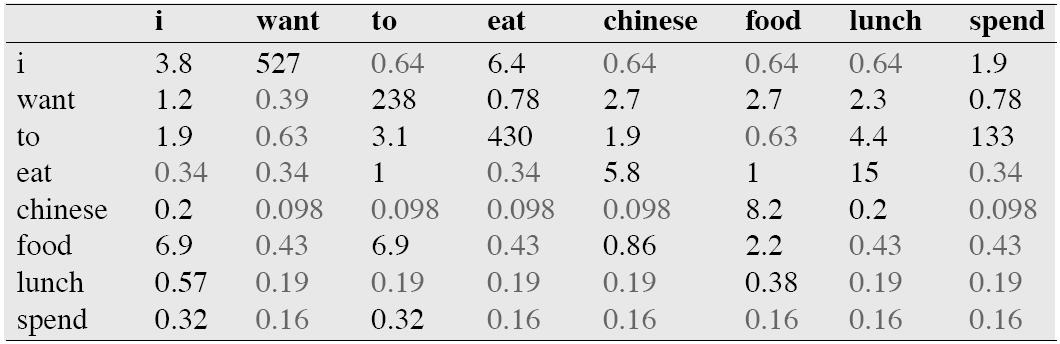
\includegraphics[width=.9\paperwidth]{ngrams4-7}	
\end{frame}

\subsection{}
\begin{frame}{Wow!  look at those counts!}

{\large Note big change to counts }

\begin{itemize}
	\item C(count to) went from 608 to 238!
	\item P(to|want) from .66 to .26!
	\item Discount d = c*/c
	\item d for `chinese food' =.10!!! A 10x reduction
	\item Laplace is a blunt instrument.
	\item But Laplace smoothing isn't used for N-grams (there are much better methods)
	\item Despite its flaws Laplace (add-k) is still used to smooth other probabilistic models in NLP, especially for pilot studies and in domains where the number of zeroes isn't so huge.
\end{itemize}
\end{frame}

\section{Evaluation}

\subsection{}
\begin{frame}{}

\begin{columns}
	\begin{column}[T]{5.5cm}
		
\includegraphics[width=5cm]{evaluation}	
	\end{column}
	
	\begin{column}[T]{3cm}
		{\Huge Evaluation}
	\end{column}
\end{columns}

\end{frame}

\subsection{}
\begin{frame}{Evaluation}

\begin{itemize}
	\item How do we know if our models are any good?
	\item And in particular, how do we know if one model is better than another.
	\item Shannon's game gives us an intuition.
	\item The generated texts from the higher order models look better. That is, they sound more like the text the model was obtained from.
	\item But what does that mean? Can we make that notion operational?
\end{itemize}
\end{frame}

\subsection{}
\begin{frame}{Evaluation}

{\large Standard method }

\begin{itemize}
	\item Train parameters of our model on a training set.
	\item Look at the models performance on some new data
	\item This is exactly what happens in the real world; we want to know how our model performs on data we haven't seen
	\item So use a test set. A dataset which is different than our training set, but is drawn from the same source
	\item Then we need an evaluation metric to tell us how well our model is doing on the test set.
	\item One such metric is perplexity (to be introduced below)
\end{itemize}
\end{frame}

\subsection{}
\begin{frame}{Evaluation}

{\large But once we start looking at test data, we'll run into words that we haven't seen before (pretty much regardless of how much training data you have). With an Open Vocabulary task:}
\vspace{.5cm}

\begin{itemize}
	\item Create an unknown word token <UNK>
	\item Training of <UNK> probabilities
	\item Create a fixed lexicon L, of size V
	\item From a dictionary or a  subset of terms from the training set
	\item At text normalization phase, any training word not in L changed to <UNK>
	\item Now we count that like a normal word
	\item At test time, use UNK counts for any word not in training
\end{itemize}
\end{frame}

\subsection{}
\begin{frame}{Evaluating N-gram models}

\begin{itemize}
	\item Put model A into an application
	\item Evaluate the performance of the application with model A
	\item Put model B into the application and evaluate
	\item Compare performance of the application with the two models
	\item This is called \textbf{Extrinsic evaluation}
\end{itemize}
\end{frame}

\subsection{}
\begin{frame}{Perplexity}

\begin{itemize}
	\item Extrinsic evaluation is really time-consuming
	\item \textbf{Perplexity} is a tool for \textbf{intrinsic evaluation}
	\item But perplexity is a poor approximation unless the test data looks just like the training data
	\item So is generally only useful in pilot experiments (generally is not sufficient to publish)
\end{itemize}
\end{frame}
\subsection{}
\begin{frame}{Perplexity}

\begin{itemize}
	\item \textbf{Perplexity} is the probability of the test set (W) (assigned by the language model), normalized by the total number of words.
	\item Minimizing perplexity is the same as maximizing probability...
	\item \textbf{The best language model is one that best predicts an unseen test set.}
\end{itemize}
\end{frame}

\subsection{}
\begin{frame}{Lower perplexity means a better model.}

\begin{itemize}
	\item Training 38 million words, test 1.5 million words, WSJ
\end{itemize}

\begin{center}
	\begin{tabular}{ | l || l | l | l | }
		\hline
		N-gram Order & Unigram & Bigram & Trigram \\ \hline
		Perplexity & 962 & 170 & 109 \\ \hline
	\end{tabular}
\end{center}
\end{frame}

\subsection{}
\begin{frame}{Skipping...}

	\begin{exampleblock}{We are skipping, for now, two big topics in smoothing...}

		\begin{description}
			\item[Backoff] Use trigram probabilities if you have them available, otherwise backoff to bigram or even unigram probabilities.
			\item[Interpolation] Mix all three levels to avoid zeroes.
		\end{description}
		
	\end{exampleblock}
\end{frame}

\subsection{}
\begin{frame}{For next time:}

     \begin{block}{For next time:}
          \begin{enumerate}
               \item Friday: \textbf{Part of Speech Tagging}
               \item Read Chapter 5 pp 123 - 139
          \end{enumerate}
     \end{block}
\end{frame}

\end{document}
